%%% Template para anotações de aula
%%% Feito por Daniel Campos com base no template de Willian Chamma que fez com base no template de Mikhail Klassen



\documentclass[12pt,a4paper, brazil]{article}

%%%%%%% INFORMAÇÕES DO CABEÇALHO
\newcommand{\workingDate}{\textsc{\selectlanguage{portuguese}\today}}
\newcommand{\userName}{DesSoftware}
\newcommand{\institution}{Universidade Positivo - Londrina}
\usepackage{researchdiary_png}




\begin{document}

\begin{center}
{\textbf {\huge Atividade pré aula 19}}\\[5mm]
{\large Desenvolvimento de Software 2023-1} \\
{\large Prof. Me. Juliana Costa Silva} \\
\today\\[5mm] %% se quiser colocar data
\end{center}
% TEMPLATE DE ATIVIDADE: https://www.overleaf.com/latex/templates/template-para-relatorio-tecnico-memorial-descritivo-utfpr/ywygvmqcqysy

\section*{Orientações}

\begin{itemize}
  \item Esta atividade tem como objetivo revisar o conceito de Interface;
  \item Utilizaremos esta atividade como "pré aula", o aluno deve desenvolve-la e tirar dúvidas na aula 19.
  \item Este não é um item pontuado (não vale pontos na média) e sim uma atividade que apoia o aprendizado do conceito visto em aula;
\end{itemize}


\vspace{0.5cm}


\section{Lanchonete}
\par

Nossa equipe de desenvolvimento foi procurada pelo dono da lanchonete DelyFood, ele precisa de um sistema para gerenciar os pedidos da lanchonete, e apresentou o seguinte cenário.
\begin{itemize}
    \item Na lanchonete servimos lanches e pizzas;
    \item Servimos bebidas, porém todas prontas (lata ou garrafa);
    \item Ao registrar um pedido preciso separar o que deve ir para a cozinha e deve ser fabricado (montado);
    \item Cada pizza possui seus ingredientes e processo de montagem, o mesmo vale para cada lanche;
    \item Ao confirmar um pedido, pode ser necessário registrar mais de uma bebida, lanche e pizza em um só pedido;
\end{itemize}

\par
A nossa equipe já modelou parte do problema, conforme apresentado no diagrama de classes abaixo:

\begin{center}
    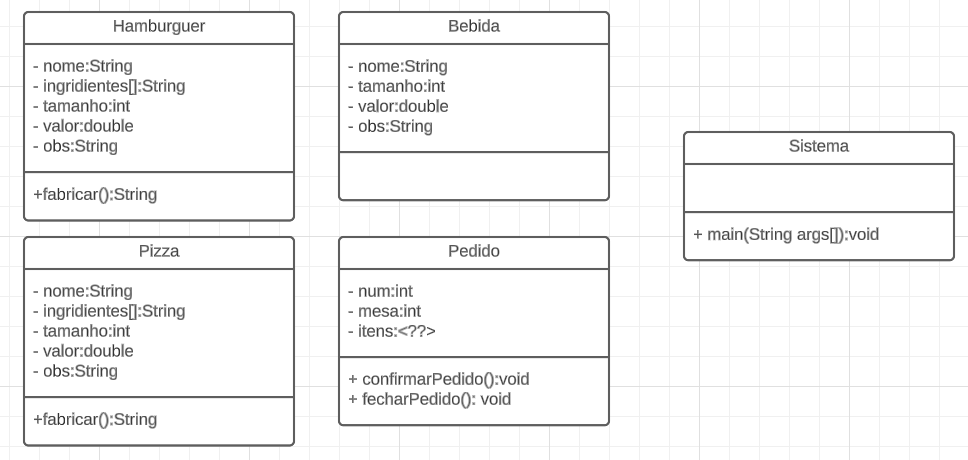
\includegraphics[width=0.7\paperwidth]{atividades/class_atv_aula18.png} \\
  \end{center}

  \par
  Porém em conversa, a professora sugeriu o uso de Interface e herança. Também disse que poderia ser necerrsário criar mais alguma classe e editar as modeladas.

  \par
  Desenvolva uma solução para o problema em linguagem Java, implementando o \textbf{Menu} da aplicação na classe sistema que permita:
  \begin{itemize}
      \item Cadastrar pizzas lanches e bebidas;
      \item Ver cardápio;
      \item Cadastrar pedidos;
      \item Listar pedidos realizados
  \end{itemize}

%%%%%%%%%%%%%%%%%% END MATTER %%%%%%%%%%%%%%%%%%
\end{document}